%%
%% This is file `example.tex',
%% generated with the docstrip utility.
%%
%% The original source files were:
%%
%% coppe.dtx  (with options: `example')
%% 
%% This is a sample monograph which illustrates the use of `coppe' document
%% class and `coppe-unsrt' BibTeX style.
%% 
%% \CheckSum{1417}
%% \CharacterTable
%%  {Upper-case    \A\B\C\D\E\F\G\H\I\J\K\L\M\N\O\P\Q\R\S\T\U\V\W\X\Y\Z
%%   Lower-case    \a\b\c\d\e\f\g\h\i\j\k\l\m\n\o\p\q\r\s\t\u\v\w\x\y\z
%%   Digits        \0\1\2\3\4\5\6\7\8\9
%%   Exclamation   \!     Double quote  \"     Hash (number) \#https://www.overleaf.com/project/5c864709d9369c09686884d3
%%   Dollar        \$     Percent       \%     Ampersand     \&
%%   Acute accent  \'     Left paren    \(     Right paren   \)
%%   Asterisk      \*     Plus          \+     Comma         \,
%%   Minus         \-     Point         \.     Solidus       \/
%%   Colon         \:     Semicolon     \;     Less than     \<
%%   Equals        \=     Greater than  \>     Question mark \?
%%   Commercial at \@     Left bracket  \[     Backslash     \\
%%   Right bracket \]     Circumflex    \^     Underscore    \_
%%   Grave accent  \`     Left brace    \{     Vertical bar  \|
%%   Right brace   \}     Tilde         \~}
%%
\documentclass[msc,numbers]{coppe}
\usepackage[T1]{fontenc}
\usepackage[utf8]{inputenc}
\usepackage[brazil]{babel}
\usepackage{amsmath,amssymb}
\usepackage[table]{xcolor}
\usepackage{hyperref}
\usepackage{natbib}
\usepackage{bm}


%%%%%%%%%%%%%%%%%%%%%%%%%%%%%%%%
%% some review tools
\usepackage{todonotes}
\usepackage{changes}
%\usepackage[disable]{todonotes} % to hide all todonotes
%\usepackage[final]{changes} % to hide all changes

% For Pedro G.
\definechangesauthor[color=orange]{PG}
\newcommand{\Padd}[1]{\added[id=PG]{#1}}
\newcommand{\Prm}[1]{\deleted[id=PG]{#1}}
\newcommand{\Pcm}[1]{\todo[color=orange!30]{PG: #1}}
%%%%%%%%%%%%%%%%%%%%%%%%%%%%%%%%



\makelosymbols
\makeloabbreviations

\begin{document}
  \title{Efeitos da corrente do Brasil na propaga\c{c}\~ao das ondas na regi\~ao sul-sudeste}
  \foreigntitle{Brazilian current effect on the southeastern region ocean wave propagation}
  % OU?
  %\foreigntitle{Brazilian current effect on the ocean wave propagation at southwest Atlantic}
  \author{Adriano}{Wiermann Barroso}
  \advisor{Prof.}{Nelson}{Violante Carvalho}{D.Sc.}

  \examiner{Prof.}{Claudio Neves}{D.Sc.}
  \examiner{Phd.}{Pedro Veras Guimaraes}{D.Sc.}
  \examiner{Phd.}{{\color{orange}ATENCAO NOME DUPLICADO}Pedro Veras Guimaraes}{D.Sc.}

  \department{PENO}
  \date{03}{2019}

  \keyword{Modelagem de ondas}
  \keyword{Intera{\c c}\~ao onda-corrente}
  \keyword{Corrente do Brasil}

  \maketitle
  \frontmatter
  %\makefrontpage

  \dedication{A algu\'em cujo valor \'e digno desta dedicat\'oria.}

  \chapter*{Agradecimentos}

  Gostaria de agradecer a todos.

  \begin{abstract}
    
    %\Padd{Os princípeos b\'asicos de intera\c{c}\~ao onda-corrente, são anteriores decada de 70 \citep{Jonsson1970,Kenyon1971}.}
    \Prm{DEIXAR PARA DEPOIS}
    \Prm{Os efeitos de correntes superficiais em ondas s\~ao amplamente conhecidos,}
    \Padd{Q}uando \Padd{ondas se propagam sobre um campo de corrent,} estas est\~ao sujeitas a um campo de correntes existe uma troca de energia entre a onda
    e a corrente. Em casos de alto cizalhamento horizontal do campo de corrente \'e
    mais not\'avel estes efeitos. O presente trabalho tem como principal objetivo 
    analisar o efeito da Corrente do Brasil no campo de ondas na regi\~ao sul-sudeste
    do Brasil. Para isso foram escolhidos alguns eventos para estudo de caso em que 
    a Corrente do Brasil apresentava estruturas de mesoescala (meandros e v\'ortices).
    Estes eventos foram simulados atrav\'es de modelagem num\'erica com o modelo de ondas
    Wave Watch III com o campo de correntes provenientes do modelo Hycom. Foram empregadas
    simula{\c c}\~oes com e sem o campo de correntes afim de verificar os impactos.
    
  \end{abstract}

  \begin{foreignabstract}
		Abstract here...
  \end{foreignabstract}

  \tableofcontents
  \listoffigures
  \listoftables
  
  \printlosymbols
  \printloabbreviations

  \mainmatter
  
  %%%%%%%%%%%%%%%%%
  %% INTRODUÇÃO  %%
  %%%%%%%%%%%%%%%%%
  \chapter{Introdu{\c c}\~ao}
  
  \Padd{Trabalhos investigando o efeito da corrente superficaila em ondas oceancas começaram a ser desernvolvidos predominantemente nos anos 60 \citep[como exemplo temos os trabalhos pioneiros de ][]{Longuet-Higgms1960,Longuet-Higgms1961}. }
  %%%%
  % \Prm{A an\'alise e modelagem num\'erica de correntes oce\^anicas e ondas foram historicamente desenvolvidas separadamente. No entanto, \'e bem conhecido os efeitos de correntes superficiais nas ondas, muitos trabalhos j\'a investigaram os efeitos que ocorrem nas ondas quando estas est\~ao sujeitas a um campo de correntes em larga escala. Trabalhos que fizeram essa an\'alise em sub e mesoescala s\~ao mais escassos, no entanto, regi\~oes como a corrente das Agulhas e corrente do Golfo j\'a foram estudados estes efeitos. Embora sejam os mesmos princ\'icios f\'isicos empregados, o impacto de correntes de menor escala ainda foi pouco explorado no oceano aberto \citet{Ardhuin2017}.} \Pcm{Vou mover isso mais para o final e dar uma editada}
  %%%%%
  \Padd{Esses trabalhos consideram que para um referêncial fixo na superície do mar sobre efeito de corrente, a relação de dispersão é modificada pelo effeito Doppler. }
%   \begin{equation}\label{eq.disp_relation}
%   \omega = \sigma + \bm{k\cdot U}
%   \end{equation}
%   \Padd{em que $\omega$ representa a frequencia absoluta da onda, $\sigma = \sqrt{gk\tanh kd}$ é a frequencia relativa dada pela relação de dispersão linear, $g$ é a gravidade e $d$ é a profundidade.  }
% 
 \Padd{Esse efeito cria uma frequencia relativa para o observador em um referencial eureliano. O efeito Doppler na propagação de ondas oceânicas já foi amplamente estudado na literatura para largas correntes ocêanicas, um exemplo é o trabalho de \citet{Mapp1985}.  }

% 
\Padd{Na presença de correntes, as propriedades intrínsicas das ondas são modificadas. Como consequência, seus comportamento advectivo e conservativos são alterados também.
\citet{Crapper1984} explora as interações não conservativas entre ondas e correntes dadas por meio das trocas de fluxos de momento, noqual onda e corrente de fato trocam energia de forma não linear. }
Segundo \Prm{conclus\~oes de} \citet{Holthuijsen}, em oceano aberto, esse efeitos de modulação das correntes locais \Padd{também} podem \Padd{modificar consideravelmente a conseração de energia das ondas,} \Prm{ser consider\'aveis,} principalmente por modificarem os processos de gera{\c c}\~ao e dissipa{\c c}\~ao de onda. \Prm{serem mais afetados nessa regi\~ao}.
	  
%	 	  \Padd{Não obstante, \citet{Crapper1984} descreve} a forma de a intera{\c c}\~ao de correntes com as ondas \'e atrav\'es de alguns mecanismos como a intera{\c c}\~ao dos fluxos de momento da corrente e da onda devida a gradientes da tens\~ao de radia{\c c}\~ao) 

\Padd{Apesar do referencial teórico já existente mostrar que os processos de interação ondas e correntes estão diretamente acoplados, a} an\'alise e modelagem num\'erica de correntes oce\^anicas e ondas \Padd{são em grande maioria tratados de forma separadas}\Prm{foram historicamente desenvolvidas separadamente}.
Muitos trabalhos investigaram \Padd{a propação das ondas sobre } \Prm{os efeitos que ocorrem nas ondas quando estas est\~ao sujeitas a} um campo de correntes em larga escala\Pcm{Citar alguns exemplos}. \Padd{No entanto,} trabalhos que fizeram essa an\'alise em sub e mesoescala s\~ao mais escassos. \Pcm{citar quem fez o trabalho na corrente das agulhas e do Golf} investigaram regi\~oes como a corrente das Agulhas e corrente do Golfo. \Prm{ j\'a foram estudados estes efeitos.} Embora sejam os mesmos princ\'icios f\'isicos empregados, o impacto de correntes de menor escala ainda foi pouco explorado no oceano aberto \citet{Ardhuin2017}.	
	
\Padd{Fenômenos de mesoescala são mais facilmente observados }\Prm{Os principais locais em que este gradiente \'e diferente de zero s\~ao} em correntes de contorno oeste pois devido a sua maior intensidade ocorre um maior cizalhamento horizontal do campo de corrente que faz com que instabilidades como meandros e v\'ortices ocorram com maior frequ\^encia\Pcm{Add referência}.
	
A Corrente do Brasil (CB)\abbrev{CB}{Corrente do Brasil}, \Padd{por exemplo, é uma} corrente de contorno oeste \Padd{que} se origina em latitudes pr\'oximas a 15$^o $S flui em dire{\c c}\~ao ao sul at\'e a regi\~ao da conflu\^encia brasil-malvinas pr\'oximo de 28$^o $S onde retroflete em dire{\c c}\~ao a \'Africa, ela se intensifica a medida que flui para baixas latitudes, com velocidades de corrente que alcan{\c c}am a ordem de 1 $m s^{-1}$ \citet{DaSilveira2008} e com intensa atividade de mesoescala reportada na literatura \citet{MILL201527}, \citet{Soutelino2011}, \citet{Mano2009}, \citet{Castelao2006}, \citet{Rodrigues2001}, \citet{Edmo2006}, \citet{Schmid95}, \citet{SIGNORINI1978481} e \citet{Mascarenhas}. Como pode ser visto na (\autoref{fig:vortice_corrente_brasil}).
  
  \begin{figure}[h]
    \centering
		\includegraphics[height=9cm]{images/rodrigues2001.png}
		\caption{Temperatura superficial do oceano imagem de sat\'etite (AVHRR-NOAA) demonstrando ressurg\^encia em Cabo Frio/RJ (cores azuis) e tamb\'em um v\'ortice quente da CB. Imagem retirada do artigo de \citet{Rodrigues2001}}
		\label{fig:vortice_corrente_brasil}
		\centering
	\end{figure}
	
  % \vspace{2 cm}
  
	Apesar da exist\^encia de uma corrente de contorno oeste intensa e com atividade de mesoescala conhecida, ainda n\~ao h\'a na literatura estudos que investiguem a influ\^encia da CB\abbrev{CB}{Corrente do Brasil} no campo de ondas na regi\~ao sul-sudeste.
  
  O clima de ondas nesta regi\~ao \Padd{é investigado por \citet{}\Pcm{Citar algém}, por meio de modelágem numérica, sem considerar o efeito das correntes na região. Segundo o mesmo, o clima de ondas é dominado por } \Prm{\'e muito caracter\'istico com persist\^encia de} vagas do quadrante leste geradas pelo AAS (Anticiclone do Atl\^antico Sul)\abbrev{AAS}{Anticiclone do Atl\^antico Sul} e a chegada de ondula{\c c}\~oes do quadrante sul com longos per\'iodos oriundas de ciclones extratropicais, apresentando a bimodalidade do mar (\autoref{fig:ilustracao_vagas_swell}) muito constante na regi\~ao \citet{Ricardo2009}, \citet{eloi2003}. 
  
  % \vspace{4 cm}
  
  \begin{figure}[h]
    \centering
		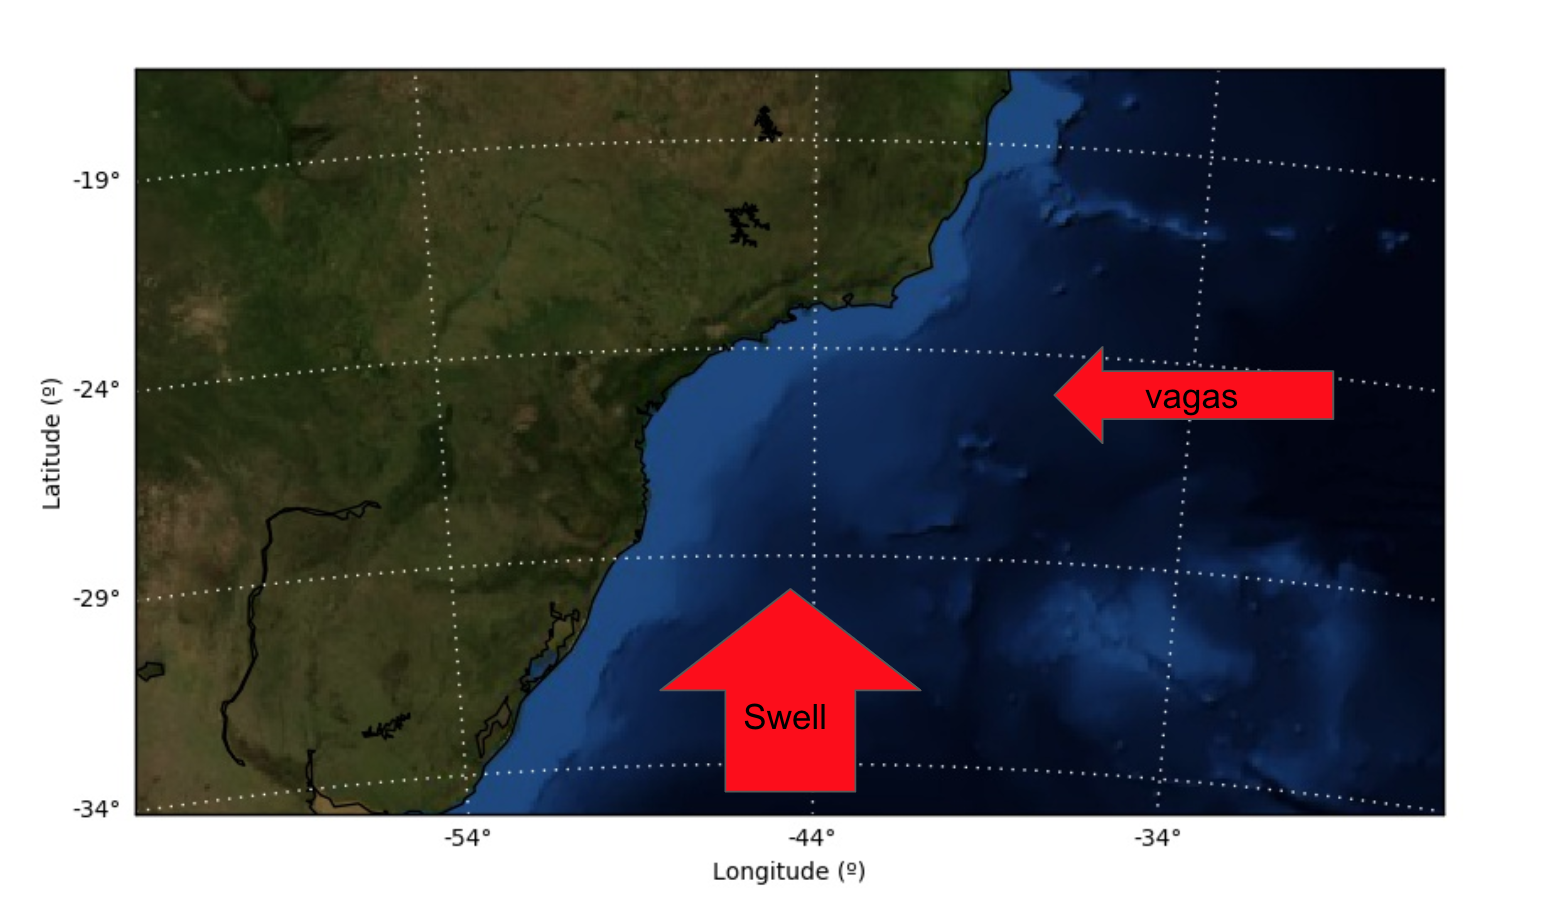
\includegraphics[height=6cm]{images/ilustracao_vagas_swell.png}
		\caption{Ilustra{\c c}\~ao da bimodalidade que ocorre na regi\~ao.}
		\label{fig:ilustracao_vagas_swell}
		\centering
	\end{figure}
  
  %A ocorr\^encia desses dois principais fatores: corrente intensa com atividade de mesoescala e \'area de gera{\c c}\~ao e propaga{\c c}\~ao de ondas evidenciam a regi\~ao da costa sul-sudeste do Brasil como potencial local em que a intera{\c c}\~ao onda-corrente se faz importante.
  \Padd{Devido a corrente intensa e alta atividade de mesoescala evidenciada na região sul-sudeste do Brasil, esta disseração tem o objetivo de investivar o comportamento e propagação das ondas sobre differentes estruturas de correntes. }
  
  \begin{figure}[h]
    \centering
		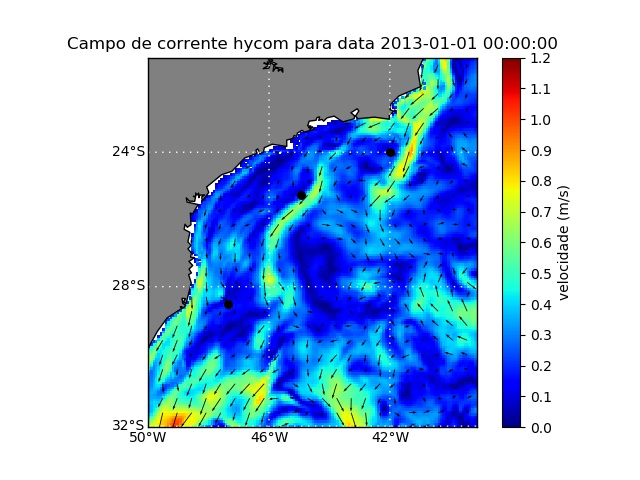
\includegraphics[height=9cm]{images/hycom_corrente_brasil.jpg}
		\caption{Campo de corrente superficial do modelo Hycom para a data de 01/01/2013. Pontos em preto representam a b\'oias do programa PNBOIA}
		\label{fig:corrente_brasil}
		\centering
	\end{figure}
  
  
  
  %%% Referencial teórico
  \chapter{Intera{\c c}\~ao Onda-Corrente}
  
  Neste cap\'itulo ser\~ao apresentados conceitos b\'asicos da intera{\c c}\~ao de um campo de ondas e corrente, bem como estudos encontrados na literatura atual.
  
  \section{Descri{\c c}\~ao das Ondas}
  
  O comprimento de onda $L$, \'e a dist\^ancia horizontal entre duas cristas de ondas sucessivas \autoref{fig:repre_onda}, e o per\'iodo $T$ \'e o tempo decorrente da passagem destas cristas ou mesmo das cavas. A frequ\^encia $f$ \'e o inverso do per\'iodo $(f = \frac{1}{T})$ , e a altura de onda $H$ \'e a dist\^ancia vertical entre uma crista e uma cava, sendo a amplitude, metade da altura $(a = \frac{H}{2})$. A profundidade local \'e representada por $h$, e $n$ representa a eleva{\c c}\~ao do n\'ivel do mar.
  
  \begin{figure}[h]
    \centering
		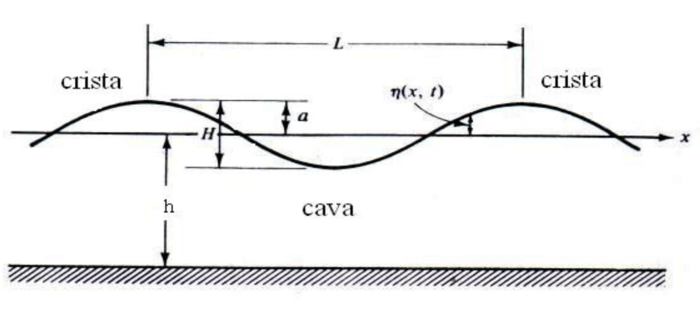
\includegraphics[height=5cm]{images/descricao_ondas.png}
		\caption{Representa{\c c}\~ao te\'orica de uma onda.}
		\label{fig:repre_onda}
		\centering
	\end{figure}
  
  A velocidade de propaga{\c c}\~ao ou velocidade de fase ($c$), \'e obtida atrav\'es da rela{\c c}\~ao de dispers\~ao das ondas representada por \citet{dean1991}:
  
  \vspace{0.5cm}
  \begin{equation}\label{eq:eq1}
    \omega^{2} = gk \tanh(kh)
  \end{equation}
  \vspace{0.5cm}
  
  onde $k$ \'e o n\'umero de onda $(k = \frac{2\pi}{L})$ e $\omega$ \'e a frequ\^encia angular $(\omega = \frac{2\pi}{T})$. A partir deles podemos representar a velocidade de fase ($c$) desta forma:
  
  \vspace{0.5cm}
  \begin{equation}\label{eq:eq2}
    c = \frac{L}{T} = \frac{\omega}{k}
  \end{equation}
  \vspace{0.5cm}
  
  e substituindo \ref{eq:eq1} em \ref{eq:eq2}, obtem-se:
  
  \vspace{0.5cm}
  \begin{equation}\label{eq:eq3}
    c = \sqrt{\frac{g}{k} \tanh(kh)}
  \end{equation}
  \vspace{0.5cm}
  
  Essa defini{\c c}\~ao da velocidade de fase ($c$) \'e importante pois nos demonstra, em \'aguas profundas ($\tanh(kh) \rightarrow 1$), que a velocidade de uma onda esta diretamente ligada ao seu comprimento $L$ que esta tamb\'em diretamente ligado ao seu per\'iodo $T$, pois substituindo os valores de $k$ e $\omega$ em \ref{eq:eq1}, obtém-se:
  
  \vspace{0.5cm}
  \begin{equation}\label{eq:eq4}
    L = \frac{gT^{2}}{2\pi} \hspace{1 cm}  ou \hspace{1 cm} L \approx 1.56T^{2}
  \end{equation}
  \vspace{0.5cm}
  
  Sendo assim, ondas com per\'iodos diferentes se propagam em velocidades de fase diferentes. E portanto, pela \ref{eq:eq3} ondas longas de maior per\'iodo se propagam mais r\'apido que ondas curtas. Isso faz com que um campo de ondas sendo gerado se organize em grupos de onda \autoref{fig:velocidade_grupo_hoj}.

  \begin{figure}[h]
    \centering
		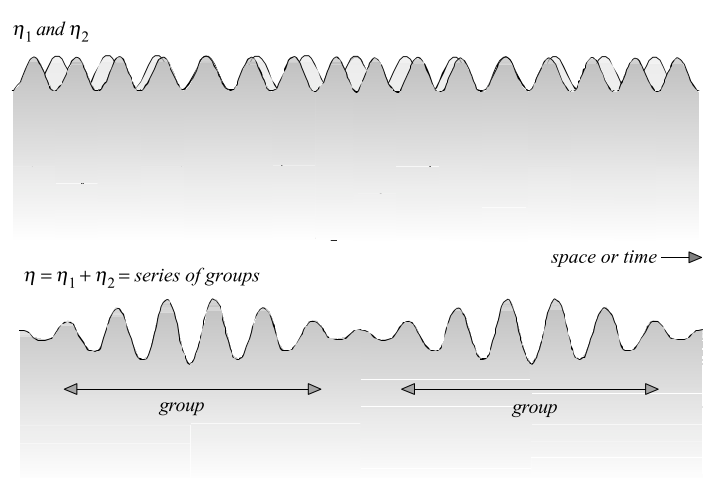
\includegraphics[height=7cm]{images/velocidade_grupo_hoj.png}
		\caption{Imagem retirada do livro de \citet{holthuijsen_2007}. Duas ondas harm\^onicas com frequ\^encias diferentes (ou n\'umero de onda) se somam criando grupos de ondas.}
		\label{fig:velocidade_grupo_hoj}		
	\end{figure}
  
  Esse grupo de ondas possui tamb\'em uma velocidade chamada de velocidade de grupo ($c_g$, eq.\ref{eq:eq5}).
  
  \vspace{0.5cm}
  \begin{equation}\label{eq:eq5}
    c_g = \frac{\partial\omega}{\partial{k}} = nc
  \end{equation}
  \vspace{0.5cm}
  
  Em que $c$ \'e a velocidade de fase da onda e $n$ \'e:
  
  \vspace{0.5cm}
  \begin{equation}\label{eq:eq6}
    n = \frac{1}{2} \left( 1 + \frac{2kh}{\sinh(2kh)} \right)
  \end{equation}
  \vspace{0.5cm}
  
  Que em \'aguas profundas se transforma em $c_{g} = \frac{1}{2}c$ pois $n = \frac{1}{2}$, ou seja a velocidade de grupo \'e metade da velocidade de uma onda individual.
  
  Enquanto as ondas viajam atrav\'es do oceano elas carregam energia com elas. S\~ao dois reservat\'orios de energia que comp\~oe a energia total, s\~ao eles a energia cin\'etica e potencial, essas duas compenentes estao representadas na \autoref{eq:eq7} derivadas a partir de aproxima{\c c}\~oes da teoria linear de onda, em que $\rho$ \'e densidade por unidade de massa e $g$ \'e a for{\c c}a da gravidade ($\thicksim9.89 m s^-2$).
  
  \vspace{0.5cm}
  \begin{equation}\label{eq:eq7}
    E_{cinetica} = \frac{1}{4}\rho g a^2 \hspace{0.5 cm} ; \hspace{0.5 cm} E_{potencial} = \frac{1}{4}\rho g a^2 \hspace{0.5 cm} 
  \end{equation}
  \vspace{0.5cm} 
  
  Seguindo o desenvolvimento de \citet{holthuijsen_2007} temos que a energia total \'e $E = E_{cinetica} + E_{potencial}$ o que resulta na \autoref{eq:eq8}.
  
  \vspace{0.5cm}
  \begin{equation}\label{eq:eq8}
      E = \frac{1}{2}\rho g a^2
  \end{equation}
  \vspace{0.5cm}
  
  E que o transporte dessa energia por unidade tempo e de crista integrado na vertical \'e,
  
  \vspace{0.5cm}
  \begin{equation}\label{eq:eq9}
    P_{energia} \hspace{0.25cm} \approx \hspace{0.25cm} \overline{\int_{-h}^{0} (p_{onda} u_x)dz} \hspace{0.25cm} = \hspace{0.25cm} (\frac{1}{2} \rho g a^2) \hspace{0.1cm} \frac{1}{2}\left( 1 + \frac{2kh}{\sinh(2hh)} \right)
  \end{equation}
  \vspace{0.5cm} 
  
  sendo que a partir da \autoref{eq:eq8} e $c = \frac{\omega}{k}$ temos:
  
  \vspace{0.5cm}
  \begin{equation}\label{eq:eq10}
    P_{energia} = Enc \hspace{0.5cm} com \hspace{0.5cm} n = \frac{1}{2}\left( 1 + \frac{2kh}{\sinh(2hh)} \right)
  \end{equation}
  \vspace{0.5cm} 
  
  Essa defini{\c c}\~ao \'e importante pois demonstra que a energia se propaga junto com a velocidade de grupo $c_g$ \ref{eq:eq5}.
  
  \vspace{0.5cm}
  \begin{equation}\label{eq:eq11}
    P_{energia} = Ec_g
  \end{equation}
  \vspace{0.5cm}
  
  A \autoref{eq:eq11} descreve o transporte de energia de uma onda. No entanto, o que acontece efetivamente no oceano \'e que temos $n$ ondas que se sobrepujam umas as outras com alturas, frequ\^encias e dire{\c c}\~oes diferentes ao mesmo tempo \autoref{fig:wave_state}. 
  
  \begin{figure}[h]
    \centering
		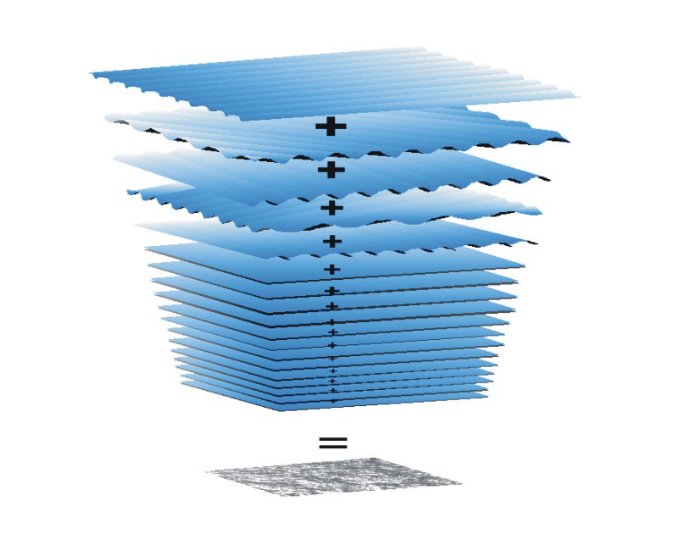
\includegraphics[height=8cm]{images/wave_state.png}
		\caption{Reconstru{\c c}\~ao de um dado estado de mar a partir da superposi{\c c}\~ao de v\'arias ondas cada uma com seu comprimento e dire{\c c}\~ao pr\'oprias. Imagem retirada do livro \citet{Ardhuin2016}.}
		\label{fig:wave_state}
	\end{figure}
  
  Por isso para representar este estado do mar utilizamos o conceito de espectro de onda que \'e basicamente uma decomposi{\c c}\~ao da eleva{\c c}\~ao do nivel do mar a partir da analise de S\'eries de Fourier em componentes sinusoidais sobrepostas, ou seja, um somat\'orio das componentes harm\^onicas das ondas registradas. Este somat\'orio de onda e seu formato pode ser descrito como:
  
  \vspace{0.5cm}
  \begin{equation}\label{eq:eq12}
    E(f) \approx g^2f
  \end{equation}
  \vspace{0.5cm}
  % e a partir de an\'alise de s\'eries de Fourier
  
  Essa descri{\c c}\~ao se faz necess\'aria pois o modelo num\'erico utilizado no presente estudo utiliza o par\^ametro de energia para suas integra{\c c}\~oes num\'ericas e propaga{\c c}\~ao das ondas.
  
  \vspace{2cm}
  
  ... Falar da dispersao e da velocidade de grupo para depois falar da propagacao de energia que a forma de calcular a propacao de onda em modelos de onda. ...
  
  \vspace{5cm}
  
  No estudo recente de \citet{Ardhuin2017} eles analisaram a influ\^encia da corrente do Golfo no campo de ondas. Pode-se verificar uma grande diferen{\c c}a no campo de ondas nas simula{\c c}\~oes com (\autoref{fig:fabrice}a) e sem corrente Golfo (\autoref{fig:fabrice}b).
  
	\begin{figure}[h]
    \centering
		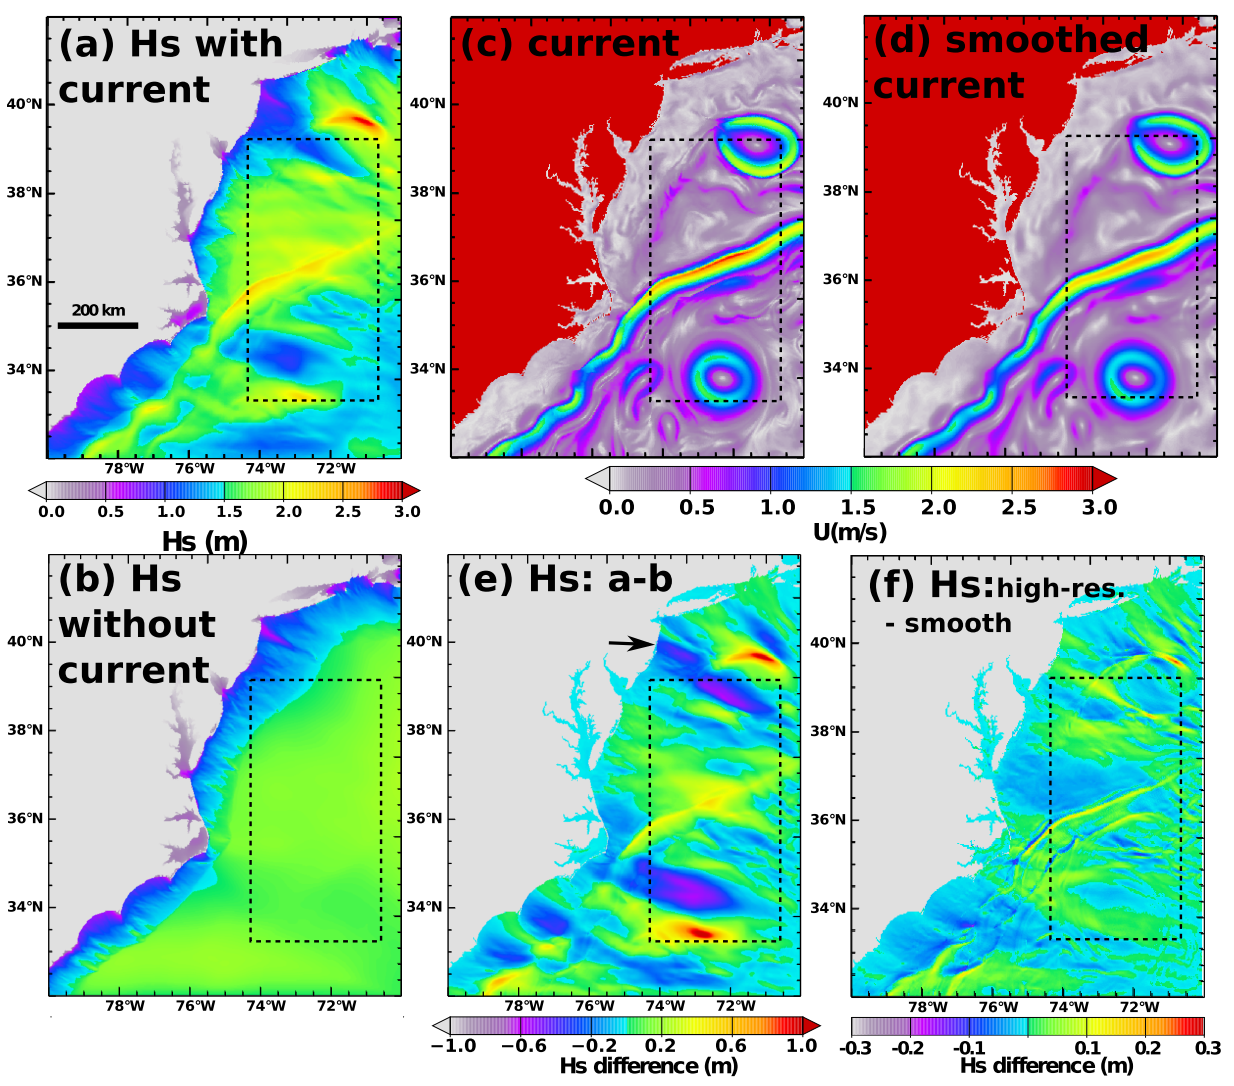
\includegraphics[height=14cm]{images/fabrice_hs.png}
		\caption{Imagem retirada do artigo citado. Impacto da corrente do Golfo nas ondas do tipo swell em 18 de Setembro de 2014, 6:00 UTC. Mapas de (a) altura de onda modelada com corrente, (b) altura de onda do modelo sem corrente, (c) corrente de alta resolu{\c c}\~ao do ROMS (d) mesma corrente filtrada. (e,f) diferen{\c c}a na altura de onda para (e) caso com corrente de alta resolu{\c c}\~ao menos caso sem corrente e (f) caso com corrente de alta resolu{\c c}\~ao menos caso com corrente filtrada. A \'area pontilhada refere-se a regi\~ao usada para an\'alise espectral.}
		\label{fig:fabrice}
	\end{figure}

  \chapter{M\'etodo Proposto}
    
  Para analisar efeitos da CB no campo de ondas foram feitas \textit{hindcasts} (simulac\~oes num\'ericas) com o modelo de ondas WW3\abbrev{WW3}{Wave Watch III} com e sem campo de corrente superficiais que foram provenientes do modelo Hycom\abbrev{Hycom}{Hybrid Coordinate Ocean Model}. Foram escolhidos eventos de alta instabilidade da CB para serem analisados.
  
  Al\'em disso foram feitas compara{\c c}\~oes com dados de boias de PNBOIA\abbrev{PNBOIA}{Programa Nacional de Boias} para o per\'iodo dos eventos modelados.
  
  \section{Simula{\c c}\~ao num\'erica}
  
  Foi feita uma simula{\c c}\~ao global com 0.5ºx0.5º de resolu{\c c}\~ao espacial durante todo o per\'iodo que compreende os eventos. Esta simula{\c c}\~ao gerou as condi{\c c}\~oes de contorno e inicias para a simula{\c c}\~ao regional que foi a utilizada para as an\'alises.
  
  Para ambas simula{\c c}\~oes foi utilizada a base batim\'etrica Etopo2, e como for{\c c}ante atmosf\'erica dados de vento do modelo ECMWF\abbrev{ECMWF}{European Centre for Medium-Range Weather Forecasts}, gentilmente cedidos pela MeteoFrance.  
  
  
  \begin{table}[h]
  \caption{Exemplos de cita{\c c}\~oes utilizando o comando padr\~ao
    \texttt{\textbackslash cite} do \LaTeX\ e
    o comando \texttt{\textbackslash citet},
    fornecido pelo pacote \texttt{natbib}.}
  \label{tab:citation}
  \centering
  {\footnotesize
  \begin{tabular}{|c|c|c|}
    \hline
    Tipo da Publica{\c c}\~ao & \verb|\cite| & \verb|\citet|\\
    \hline
    Livro &  & \\
    Artigo &  & \\
    Relat\'orio &  & \\
    Relat\'orio &  & \\
    Anais de Congresso &  &
      \\
    S\'eries &  & \\
    Em Livro &  & \\
    Disserta{\c c}\~ao de mestrado &  &
      \\
    Tese de doutorado &  & \\
    \hline
  \end{tabular}}
  \end{table}
    
  \begin{itemize}
		\item Coeficiente de Correla{\c c}\~ao (r):
		\begin{equation}\label{eq:teste}
			r = \frac{\sum_{i=1}^n (m_i - \bar{m})(o_i - \bar{o})}
							 {\sqrt{ \left(\sum_{i=1}^n (m_i - \bar{m})^2 \sum_{i=1}^n (o_i - \bar{o})^2 \right)}}
		\end{equation}
	\end{itemize}
  
  \chapter{Resultados e Discuss\~oes}
  \chapter{Conclus\~oes}

  \backmatter
  \bibliographystyle{coppe-unsrt}
  % \bibliographystyle{unsrtnat}
  %\bibliographystyle{apa}
  % \bibliographystyle{unsrtnat}
  % \bibliographystyle{coppe-unsrt}
  \bibliography{mestrado}

  \appendix
  \chapter{Algumas Demonstra{\c c}\~oes}
\end{document}
%% 
%%
%% End of file `example.tex'.
